


% Dokumentenklasse
\documentclass[a4paper,12pt,liststotoc, parskip=half]{scrreprt}

    % ============ Pakete ============
    % Dokumentinformationen

    % FONTS
    \usepackage[utf8]{inputenc}
    \usepackage[ngerman]{babel}
    \usepackage[T1]{fontenc}
    \usepackage{fancyhdr}
    \usepackage{graphicx}
    \usepackage{lmodern}
    \usepackage{color}
    \usepackage{booktabs}
    \usepackage[onehalfspacing]{setspace}
    \usepackage{geometry}
    \usepackage{authblk}
    \usepackage{longtable}
    \usepackage{amsfonts}
    \usepackage{amsmath}
		\usepackage{pdfpages}
		\usepackage{hyperref}
    \usepackage[ngerman, nameinlink, noabbrev]{cleveref}

    % C++ Code Gedöns
    \usepackage{listings}
    \lstset{numbers=left, numberstyle=\tiny, numbersep=5pt}

    % Fortlaufende nummerierung
    \usepackage{chngcntr}
    \counterwithout{figure}{chapter}
    \counterwithout{table}{chapter}
		\usepackage{ulem}
		\usepackage{fancybox}
    % Style
    \pagestyle{fancy}
		\renewcommand{\footrulewidth}{0.2pt}		% Dünne Trennline vor der Fußzeile
		\hyphenation{De-zi-mal-tren-nung}
    \hyphenation{Ent-wick-lung}
    \hyphenation{ent-wick-eln}
    \hyphenation{Library}
		\usepackage{mathptmx}
    \usepackage{helvet}

		\newcommand{\scl}{\begin{lstlisting}}

		\newcommand{\ecl}{\end{lstlisting}}
    \begin{document}
    \pagestyle{fancy}

    \title{
      Funktionale und Objektorientierte Programmierung
      \large ---- \\ Dieses Skript richtet sich nach der Vorlesung von \\ Prof. Dr. rer. nat. Karsten Weihe \\ Formulierungen sind teils von den Folien übernommen.}
		\author{}
    \date{\today}
    \affil{Technische Universität Darmstadt}
    \maketitle
    \pagestyle{fancy}
    % Kopfzeile
    \lhead{}
    \chead{\leftmark}
    \rhead{}

    % Fußzeile
    \lfoot{FOP}
    \cfoot{\thepage}
    \rfoot{ %\slshape
    \date{\today} }

    % Inhaltsverzeichnis
    \begingroup
      \renewcommand*{\chapterpagestyle}{empty}

      \pagestyle{empty}
      \tableofcontents
      %\clearpage
    \endgroup

    \pagenumbering{Roman}

    \clearpage
    \pagenumbering{arabic}

    % Kapitel einbinden
    
\chapter{Grundlagen der Programmierung}
\label{c:grundlagen}
\setcounter{page}{1}
\section{Was ist Progrmamieren?}

Schauen wir zunächsteinmal, was einige der „großen Köpfe“ der
Informatik das Programmieren definieren.

\begin{quote}
	„To program is to understand“ \\
	\textit{~ Kristen Nygaard}
\end{quote}

\begin{quote}
	„Programming is a Good Medium for Expressing Poorly
	Understood and Sloppily Formulated Ideas“\\
	\textit{~ Marvin Minsky, Gerald J. Sussman}
\end{quote}

Eine Programmiersprache ist mehr als ein Hilfsmittel um einen
Computer anzuweisen, Aufgaben durchzuführen. 
Sie dient auch als \textbf{Rahmen}, innerhalb dessen wir \textbf{unsere
Ideen} über die \textbf{Problemdomäne organisieren.}

Wenn wir eine Sprache beschreiben, sollten wir
die Hilfsmittel beachten, die sie uns zum
Kombinieren von einfachen Ideen anbietet, um
komplexere Ideen zu bilden.

Jede vollwertige Programmiersprache hat drei Mechanismen,
um Prozessideen zu strukturieren:

\begin{itemize}
	\item \textbf{\textit{Primitive} Ausrücke}
		\subitem - Repräsentieren die einfachsten Einheiten der Sprache
		\subitem - Im Deutschen: jedes Wort ist ein primitiver Ausdruck
	\item \textbf{\textit{Kombinationsmittel}}
		\subitem - Zusammengesetzte Elemente werden aus einfacheren Einheiten
		konstruiert
		\subitem - Im Deutschen: Zusammensetzung mehrerer Wörter zu einem Satz.
	\item \textbf{\textit{Abstraktionsmittel}}
		\subitem - Zusammengesetzte Elemente können benannt und weiter als Einheiten manipuliert werden
		\subitem - Im Deutschen: Definition eines Begriffs („Ein Auto ist ...“), so dass der Begriff danach als „Kurzform“ für die Erklärung nutzbar ist
\end{itemize}

\textbf{Strukturierungsmechanismen in der Elektronik:}

\begin{itemize}
	\item \textbf{\textit{Primitive} Ausrücke}
		\subitem - Widerstände, Kondensatoren, Induktivitäten, Spannungsquellen, ...

	\item \textbf{\textit{Kombinationsmittel}}
		\subitem - Richtlinien für das Verdrahten der Schaltkreise
		\subitem - Standardschnittstellen (z.B. Spannungen, Strömungen) zwischen den
		Elementen. Diese Schnittstellen können auch Anforderungen an
		konkrete zulässige Werte oder Einheiten stellen („5 mA“)
		
	\item \textbf{\textit{Abstraktionsmittel}}
		\subitem - 	“Black box” Abstraktion – denke über einen Unter-Schaltkreis als eine
		Einheit: z.B. Verstärker, Regler, Empfänger, Sender, ...
\end{itemize}



    \section{Formales}

    \chapter{Strukturierte Datentypen}

    \chapter{Rekursive Datentypen und Strukturelle Rekursion}
\section{Listen}
Mit Strukturen können Datenobjekte mit einer festen Zahl von Daten gespeichert werden. Häufig wissen wir jedoch nicht, aus wie vielen Datenelementen eine Datenstruktur besteht.
%%%%%%%%%%%%%%%%%%%%%%%%%%%%%%%%%%%%%%%%%%%
Oder die Struktur der Daten ist rekursiv.
%???? KEINE AHNUNG WAS MIT DEM LETZTEN SATZ GEMEINT IST!!!
Mit rekursiven Datentypen können auch beliebig große Datenobjekte strukturiert abgespeichert werden. Die Idee davon ist die Folgende: Ein Element der Datenstruktur speichert (direkt oder indirekt) ein Exemplar der Datenstruktur. Dies nennt man dann eine \textit{rekursive Datenstruktur}. Um eine \uline{endliche} Datenstruktur zu bekommen benötigt man einen \textit{Rekursionsanker}. Diesen Rekursionsanker modellieren wir mit der Technik zu heterogenen Daten aus dem letzten Kapitel.

Eine Liste ist entweder die leere Liste \textit{the-emtpylst}, oder \textit{(make-lst s r)}, wobei s ein Wert ist und r eine Liste. Im folgenden sehen wir eine Modellierung von Listen mit Struktur.

\begin{lstlisting}{t03-prog1}
;; a list with 0 elements
;; (define list0 the-emptylst)
(define list0 empty)

;; a list with 1 element
;; (define list1 (make-lst 'a the-emptylst))
(define list1 (cons 'a empty))

;; a list with 2 elements
;; (define list2 (make-lst 'a
;;               (make-lst 'b the-emptylst)))
(define list2 (cons 'a (cons 'b empty)))

;; get the 2nd element from list2
;; (lst-first (lst-rest list2)) -> 'b
(first (rest list2)) ;; -> 'b
\end{lstlisting}

Listen sind ein wichtiger Datentyp, weshalb es einen eingebauten Datentyp existiert. Der Konstruktor \textit{cons} besitzt zwei argumente. cons entspricht unserem \textit{make-lst} Eigenbeispiel und steht wie es leicht zu vermuten ist für \textit{cons}truktor. Zudem existiert eine leere Liste \textit{emtpy} die unserer leeren Liste \textit{the-emptylst} entspricht. Auf die Sektoren der Liste kann man mit \textit{first} und \textit{rest} zugreifen. Mit \textit greift man auf das erste Element und mit \textit{rest} auf den Rest der Liste zu. Zudem haben beide noch \textit{historische Namen} die da lauten \textit{car} für \textit{first} und \textit{cdr} für rest. Die Prädikate \textit{lst?} und \textit{emtpy?} entsprechen \textit{lst?} und \textit{emptylst?}.
\textit{lst?} checkt ob es eine Liste ist und \textit{emptylst?} ob die Liste leer ist. Im Folgenden nun ein Beispiel:


\begin{lstlisting}{t03-prog2}
; a list with 0 elements
;; (define list0 the-emptylst)
(define list0 empty)

;; a list with 1 element
;; (define list1 (make-lst 'a the-emptylst))
(define list1 (cons 'a empty))

;; a list with 2 elements
;; (define list2 (make-lst 'a
;;               (make-lst 'b the-emptylst)))
(define list2 (cons 'a (cons 'b empty)))

;; get the 2nd element from list2
;; (lst-first (lst-rest list2)) -> 'b
(first (rest list2)) ;; -> 'b
\end{lstlisting}

Wie sie sehen besteht der einzige Unterschied zwischen \textit{make-lst} und \textit{cons} darin, dass \textit{cons} als zweites argument \textit{empty} oder \textit{(cons ...)}. Zum Beispiel :

\begin{lstlisting}{t03-prog3}
(cons 1 2)
\end{lstlisting}
ist ein Fehler
\begin{lstlisting}{t03-prog3}
(make-lst 1 2)
\end{lstlisting}
aber nicht.\\
\textit{cons} verhindert also inkorrekte Nutzung der Prozedur. In anderen LISP-basierten Dialekten fehlt allerdings diese Überprüfung. \\\\
Eine bessere Emulation sähe wie folgt aus:

\begin{lstlisting}{t01-prog4}
(define-struct lst (first rest))
(define-struct emptylst ())
(define the-emptylst (make-emptylst))
(define (our-cons a-value a-list)
  (cond
    [(emptylst? a-list) (make-lst a-value a-list)]
    [(lst? a-list) (make-lst a-value a-list)]
    [else (error 'our-cons "list as second argument expected")]))
\end{lstlisting}
Dies kann aber nicht verhindern, dass man \textit{make-lst} direkt verwendet. Im folgenden noch einige visuelle Beispiele.

\begin{lstlisting}{t03-prog4}
(cons 'Mercury empty)
\end{lstlisting}
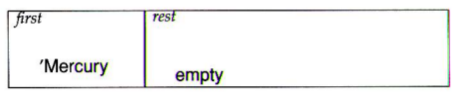
\includegraphics[height=2cm]{Bilder/T03_00.png}

\begin{lstlisting}{t03-prog4}
(cons 'Venus
    (cons 'Mercury empty))
\end{lstlisting}
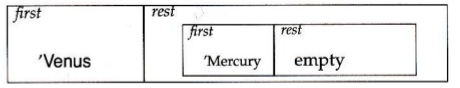
\includegraphics[height=2cm]{Bilder/T03_01.png}

\begin{lstlisting}
(cons 'Earth
  (cons 'Venus
	  (cons 'Mercury empty)))
\end{lstlisting}
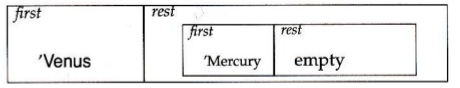
\includegraphics[height=2cm]{Bilder/T03_01.png}

In den folgenden Beispielen sehen wir: Listen speichern beliebige Datentypen, auch gemischte Daten.

\begin{lstlisting}{t03-prog5}
(cons 0
  (cons 1
    (cons 2
      (cons 3
        (cons 4
      	  (cons 5
            (cons 6
              (cons 7
                (cons 8
                  (cons 9 empty))))))))))
\end{lstlisting}

\begin{lstlisting}{t03-prog6}
(cons 'RobbyRound
  (cons 3
    (cons true empty)))
\end{lstlisting}
%%% ###########################################
\section{Abgeschlossenheitseigenschaft}
Eine Operation zum Kombinieren von Daten besitzt die Abgeschlossenheitseigenschaft, wenn die Ergebnisse der Kombination von Datenobjekten wiederum mit der Operation kombiniert werden können.  \textit{cons} ist hier ein gutes Beispiel. Solche Kombinationsoperatoren können verwendet werden, um hierarchische Daten aufzubauen. \\\
Doch sind wir der Abgeschlossenheit schon einmal begegnet?\\
Der Ursprung des Begriffs „Abgeschlossenheit“ (engl. closure) kommt aus der abstrakten Algebra. Es gilt:
\begin{quote}
	Eine Menge von Elementen ist abgeschlossen bezüglich einer Operation, wenn die Anwendung der Operation an Elementen der Menge wieder ein Element der Menge produziert.
\end{quote}
Der Gedanke, dass ein Mittel der Kombination die Abgeschlossenheitseigenschaft besitzen soll, ist intuitiv, jedoch erfüllen Kombinationsoperatoren vieler Programmiersprachen diese nicht. So kann man Elemente kombinieren, indem man diese in Arrays (->T11.84ff) speichert. Man kann aber unter Umständen keine Arrays aus Arrays zusammenstellen bzw. als Rückgabewerte von Prozeduren verwenden. Es fehlt ein eingebauter „Universalkleber“, der es einfacher macht, zusammengesetzte Daten in einer uniformen Art und Weise zu manipulieren.

\section{list Konstruktor}
Längere Listen mit \textit{cons} zu erzeugen ist unhandlich, daher gibt es in den HtDP-TL den Konstruktor \textit{list}. Dieser bekommt eine beliebige Menge von Argumenten und erzeugt eine Liste mit allen Argumenten als Elementen. Als Beispiel:

\begin{lstlisting}{t03-prog7}
(list 1 2 3)
\end{lstlisting}
statt
\begin{lstlisting}{t03-prog7}
(cons 1 (cons 2 (cons 3 empty)))
\end{lstlisting}
oder zum Beispiel:
\begin{lstlisting}{t03-prog8}
(list (list 'a 1) (list 'b 2))
\end{lstlisting}

Allgemein gilt
\begin{lstlisting}{t03-prog9}
(list exp-1 ... exp-n)
\end{lstlisting}
 äquivalent zu
\begin{lstlisting}{t03-prog9}
(cons exp-1 (cons ... (cons exp-n empty))...)
\end{lstlisting}

\section{Der ' oder quote Konstruktor}
Da Listen wirklich sehr oft eingesetzt werden können einige Listen können mit Hilfe des Quote-Konstruktors ' noch weiter abgekürzt werden.
\begin{lstlisting}{t03-prog10}
'(1 2 3)
\end{lstlisting}
ist die Kurzform für
\begin{lstlisting}{t03-prog10}
(list 1 2 3)
\end{lstlisting}
Ein weiteres Beispiel:
\begin{lstlisting}{t03-prog11}
'((1 2) (3 4) (5 6))
\end{lstlisting}
steht für
\begin{lstlisting}{t03-prog11}
(list (list 1 2) (list 3 4) (list 5 6))
\end{lstlisting}
dies sollte man nicht verwechseln mit (list a b c) – list wertet alle
Argumente aus, quote jedoch nicht. \\Im Allgemeinen bedeutet also
\begin{lstlisting}{t03-prog12}
'(e-1 ... e-n)
\end{lstlisting}
steht für
\begin{lstlisting}{t03-prog12}
(list 'e-1 ... 'e-n)
\end{lstlisting}
Achtung:\\
\textit{'exp-i} ist ein Symbol, wie z.B. \textit{'+'}, \textit{'true}, \textit{'list (!!!)}. Nur für Zahlen gilt \textit{'e-i = e-i}. Beachten Sie, dass diese Regel rekursiv ist! Um list und quote zu verwenden, stellen Sie ab jetzt DrRacket um auf den Sprachlevel “Beginning Student with List Abbreviations” bzw. „Anfänger mit Listen-Abkürzungen“!

\section{Verarbeitung rekursiver Datentypen}
Jetzt kann man sich die Frage stellen wie wir nun unsere Exemplaren rekursiven Datentypen? Die Antwort ist simpel: Wir benutzen unser Designrezept für heterogene Daten.\\

1. Schritt: Definition des Vertrags, Header etc. \\
Beachten Sie die Konvention (listof XXX), um im Vertrag zu dokumentieren, \\
was für Daten als Listenelemente erwartet werden.
\begin{lstlisting}{t03-prog13}
;; contains-doll?: (listof symbol) -> boolean
;; to determine whether the symbol 'doll occurs
;; in a-list-of-symbols
(define (contains-doll? a-list-of-symbols) ...)
\end{lstlisting}

2. Schritt: Tabelle erstellen:\\
Für jeden Datentyp ein cond-Zweig u. Selektoren andeuten\\
\begin{lstlisting}[firstnumber=4]
(define (contains-doll? a-list-of-symbols)
  (cond
    [(empty? a-list-of-symbols) ...]
    [(cons? a-list-of-symbols)
        ... (first a-list-of-symbols) ...
        ... (rest a-list-of-symbols) ...]))
\end{lstlisting}
Der Erster Fall (leere Liste) ist trivial
\begin{lstlisting}[firstnumber=6]
[(empty? a-list-of-symbols) false]
\end{lstlisting}

Mit den verfügbaren Daten können wir direkt das erste Element
der Liste überprüfen.

\begin{lstlisting}[firstnumber=7]
[(cons? a-list-of-symbols)
  (cond
    [(symbol=? (first a-list-of-symbols) 'doll) true]
    ... (rest a-list-of-symbols) ...]))
\end{lstlisting}
Was machen wir mit dem Rest der Liste? Wir brauchen eine Hilfs-Prozedur, die überprüft, ob die (Rest)-Liste das Symbol enthält. Für die Hilfsprozedur nehmen wir \textit{contains-doll?} einfnach selbst. Der folgende Codeteil ist die Lösung.

\begin{lstlisting}
(define (contains-doll? a-list-of-symbols)
  (cond
    [(empty? a-list-of-symbols) false]
    [(cons? a-list-of-symbols)
      (cond
        [(symbol=? (first a-list-of-symbols) 'doll) true]
        [else (contains-doll? (rest a-list-of-symbols))])]))
\end{lstlisting}

Hier könnte man sich fragen: Wieso ist die Lösung wohldefiniert? (Wohldefiniert bedeutet hier: "die Ausführung der Prozedur endet") Denn nicht jede rekursive Definition ist wohldefiniert z.B.:
\begin{lstlisting}
(define (f a-bool) (f (not a-bool)))
\end{lstlisting}
Unsere rekursive Definition ist ein Beispiel für strukturelle
Rekursion, da Sie Struktur der Prozedur der (rekursiven) Struktur der Daten folgt. Solche rekursiven Definitionen sind stets wohldefiniert, weil die Schachtelungstiefe der Daten in jedem rekursiven Aufruf strikt abnimmt.

\section{Design von Prozeduren für rekursive Daten}
Wie ändert sich also nun unser Designrezept? In der \textbf{Datenanalyse und im Design} ändert ich das folgende: Wenn die Problembeschreibung Informationen beliebiger Größe beschreibt, benötigen wir eine rekursive Datenstruktur. Diese Datenstruktur benötigt mindestens zwei Fälle, von denen mindestens einer weder direkt noch indirekt auf die Definition zurückverweist – also eben \textit{nicht} rekursiv ist. Im \textbf{Template} müssen die rekursiven Zweige den rekursiven Aufruf andeuten. Im \textbf{Prozedurkörper} werden erst die \textit{Basisfälle} (nicht-rekursiv) implementieren, dann die rekursiven Zweige. Für die rekursiven Aufrufe davon ausgehen, dass die Prozedur bereits wie gewünscht funktioniert. Sonst ändert sich nichts weiteres.

\section{Erzeugen von rekursiven Daten}
Prozeduren, die rekursive Daten nach unserem Designrezept verarbeiten, kombinieren üblicherweise die Lösung aus den rekursiven Aufrufen mit den nicht-rekursiven Daten. Diese Kombination besteht häufig in der Konstruktion neuer Daten, deren Struktur analog zu denen der Eingabe ist.
\begin{lstlisting}
(define (sum a-list-of-nums)
  (cond
    [(empty? a-list-of-nums) 0]
    [else (+
  (first a-list-of-nums)
  (sum (rest a-list-of-nums)))]))
\end{lstlisting}

Im folgenden Beispiel wird ein Programm zur Lohn für eine oder mehr Personen. Die Schreibweise mit dem "Pfeil" im Namen ist eine Konvention, wenn Werte "umgerechnet" werden. Sie hat \textit{eigene} Semantik.
\begin{lstlisting}
;; wage : number -> number
;; to compute the total wage (at $12 per hour)
;; of someone who worked for h hours
(define (wage h)
  (* 12 h))
;; hours->wages : (listof number) -> (listof number)
;; to create a list of weekly wages from
;; a list of weekly hours (alon)
(define (hours->wages alon)
  (cond
    [(empty? alon) empty]
		[else (cons
      (wage (first alon))
      (hours->wages (rest alon)))]))
\end{lstlisting}

\section{Strukturen die Strukturen enthalten}
Strukturen (und Listen) müssen nicht notwendigerweise atomare Daten enthalten. Sie können z.B. Exemplare ihrer eigenen Struktur als Elemente (wie bei der Listenstruktur), aber auch beliebige andere Strukturen/Listen enthalten. Sie können z.B. auch Exemplare ihrer eigenen Struktur als Elemente enthalten (wie bei der Listenstruktur). Zudem können sie beliebige andere Strukturen/Listen enthalten z.B. Liste von Punkten, Liste von Listen von Punkten. Hier ein kleines Beispiel:

Ein Inventareintrag ist eine Struktur \textit{(make-ir s n)}, wobei s ein Symbol ist und n eine (positive) Zahl:
\begin{lstlisting}
(define-struct ir (name price))
\end{lstlisting}
Eine Inventarliste ist entweder \textit{empty} leer, oder \textit{(cons ir inv)}, wobei ir ein Inventareintrag ist und inv eine \textit{Inventarliste}.

\subsection{Die Struktur natürlicher Zahlen}
Natürliche Zahlen werden häufig als Aufzählungen eingeführt: 0,1,2 etc. Jedoch ist dieses "etc." nicht besonders hilfreich für die Programmierung. Mit Hilfe einer rekursiven Definition kann man das "etc." los werden:
0 ist eine natürliche Zahl und falls n eine natürliche Zahl ist, dann auch der Nachfolger (succ n). Diese Definition generiert also
\begin{lstlisting}
(0, (succ 0), (succ (succ 0))
\end{lstlisting}
usw. Vergleichbar ist dies mit den Peano-Axiomen in der Mathematik. Diese Konstruktion ist analog zu der Konstruktion von Listen.

\begin{itemize}
	\item \textbf{cons} entspricht \textit{succ}
	\item \textbf{rest} entspricht \textit{pred}
	\item \textbf{empty?} entspricht \textit{zero?}
\end{itemize}
Funktionen auf natürlichen Zahlen können daher analog zu Funktionen auf Listen strukturiert werden. Hier die Definition der Prozeduren pred, succ und zero?:

\begin{lstlisting}
;; pred: N -> N
;; returns the predecessor of n; if n is 0, return 0
(define (pred n)
  (if (> n 0)
    (- n 1)
      0))
;; succ: N -> N
;; returns the successor of n; if negative, return 0
(define (succ n)
  (if (>= n 0)
    (+ n 1)
      0))
;; zero?: N -> boolean
;; returns true if N is 0, else false
;; Already defined in HtDP-TL, no need to do it again!
\end{lstlisting}

Beispiel 1:
\begin{lstlisting}
;; hellos : N -> (listof symbol)
;; to create a list of n copies of 'hello
(define (hellos n)
  (cond
    [(zero? n) empty]
    [else (cons 'hello (hellos (pred n)))]))
\end{lstlisting}

Beispiel 2:
\begin{lstlisting}
;; ! : N -> N
;; computes the faculty function
(define (! n)
  (cond
    [(zero? n) 1]
    [else (* n (! (pred n)))]))
\end{lstlisting}

\section{Intermezzo: Design von Hilfsprozeduren}
\subsection{Wunschlisten)}
Größere Programme bestehen aus vielen verschiedenen
(Hilfs-)Prozeduren. Ein sinnvolles Vorgehen hierbei ist das Anlegen und Pflegen einer Wunschliste von Hilfsprozeduren. Eine Wunschliste ist eine Liste der Prozeduren, die noch entwickelt werden müssen, um ein Programm fertigzustellen. Die Prozeduren auf der Wunschliste können wir dann schrittweise mit Hilfe der Designrezepte implementieren. So eine Wunschliste ändert sich häufig im Laufe der Implementierung, etwa weil man entdeckt, dass bestimmte neue Hilfsprozeduren erforderlich sind um andere Prozeduren zum aufen zu bekommen. Die Reihenfolge der Abarbeitung der Wunschliste ist wichtig. Es gibt zwei Lösungsansetze die die Abarbeitung für den Entwickler vereinfachen. \\
\subsubsection{"Bottom-Up"-Ansatz:}
Hier werden erst die Prozeduren implementieren, die von keiner anderen Prozedur auf der Wunschliste abhängen.\\Der Vorteil: Wir können sofort und jederzeit testen\\
Der Nachteil: Am Anfang ist oft noch nicht klar, welche Prozeduren auf
der untersten Ebene benötigt werden; es kann der Gesamtüberblick
verloren gehen
\subsubsection{"Top-Down"-Ansatz:}
Hier wird erst die Hauptprozedur implementieren, dann die dort aufgerufenen Funktionen usw.
\\Vorteil: Inkrementelle Verfeinerung der Programmstruktur
\\Nachteil: Man kann erst sehr spät testen; manchmal findet man erst “unten” einen konzeptuellen Fehler "oben". \\
\\Oft ist aber eineMischung aus Top-Down und Bottom-Up sinnvoll. Hier nun ein Beispiel zum Sortieren einer Liste von Zahlen. Aka. "Insertion Sort"
\begin{lstlisting}
;; sort : (listof number) -> (listof number)
;; to create a sorted list of numbers from all
;; the numbers in alon
;; Examples:
;;(sort empty) -> empty
;; (sort (cons 1297.04 (cons 20000.00 (cons -505.25 empty))))
;; -> (cons -505.25 (cons 1297.04 (cons 20000.00 empty)))
(define (sort alon)
  (cond
    [(empty? alon) ...]
    [else ... (first alon) ... (sort (rest alon)) ...]))
\end{lstlisting}

Der erste Fall (leere Liste) ist trivial. Der Aufruf \textit{(sort (rest alon))} im rekursiven Fall gibt uns eine sortierte Liste zurück. In diese Liste muss \textit{(first alon)} einsortiert werden. Die Prozedur, die dies erledigt, kommt auf unsere Wunschliste,
die \textit{sort}-Prozedur können wir schon mal komplettieren.

\begin{lstlisting}
;; insert : number (listof number) -> (listof number)
;; to create a list of numbers from n and the numbers
;; in alon that is sorted in descending order; alon is
;; already sorted
(define (insert n alon) ...)
(define (sort alon)
  (cond
    [(empty? alon) empty]
    [else (insert (first alon) (sort (rest alon)))]))
\end{lstlisting}
Die \textit{insert}-Prozedur kann nun unabhängig von sort
implementiert werden. Hierbei ist genaue Analyse der unterschiedlichen Fälle wichtig.
\begin{lstlisting}
;; insert : number (listof number) (sorted)
;;              -> (listof number) (sorted)
;; to create a list of numbers from n and the numbers in
;; alon that is sorted in ascending order; alon is sorted
(define (insert n alon)
  (cond
    [(empty? alon) (cons n empty)]
    [else (cond
    [(<= n (first alon))(cons n alon)]
    [(> n (first alon))(cons
        (first alon)(insert n (rest alon)))])]))
\end{lstlisting}
\subsection{Verallgemeinerung von Problemen}
Häufig ist ein allgemeineres Problem als das, was man eigentlich lösen möchte einfacher zu verstehen als das eigentliche Problem. Die Abstraktion kann also durchaus die Lösung leichter machen. \\\\
Doch wie gehen wir hier vor? Die Hilfsprozedur löst ein allgemeineres Problem, doch Hauptprozedur spezialisiert die Hilfsprozedur für das eigentliche Problem.
Als Beispiel nehmen wir einen Münzwechsel. \\\\
Auf wie viele Arten kann man einen Euro-Betrag a wechseln (unter Verwendung von Münzen à 1,2,5,10,20,50 Cent)? Verallgemeinern wir das Problem zunächst. Auf wie viele Arten kann man einen Euro-Betrag a wechseln, unter Verwendung der ersten n Münzarten aus 1,2,5,10,20,50 Cent? Spezialisieren wir: n=6\\\\
Wichtig ist es, dass die Formulierung es allgemeinen Problems als rekursive Prozedur einfach erklärt wird.\\\\
Die Anzahl der Möglichkeiten den Betrag a unter Verwendung von n Sorten von Münzen zu wechseln, ist:

\begin{itemize}
	\item $1 \text{f alls } a = 0$
\end{itemize}

		\chapter{Auswertungsreihenfolge und Lexikalisches Scoping}

\section{Intermezzo: Syntax und Semantik der HtDP-TL}

\subsectiom{Syntax}
Ähnlich wie die natürlichen Sprachen haben auch die
Programmiersprachen ein Vokabular und eine Grammatik. Das Vokabular ist eine Sammlung der "Wörter", aus denen wir Sätze" in unserer Sprache bilden können. Ein Satz in einer Programmiersprache ist ein Ausdruck oder eine Funktion. Die Grammatik der Sprache sagt uns, wie wir ganze Sätze aus Wörtern bilden. Der Ausdruck Syntax bezieht sich auf Vokabular und Grammatik von Programmiersprachen.

\subsection{Semantik}

Nicht alle grammatikalisch richtigen Sätze sind sinnvoll, weder in Deutsch noch in Programmiersprachen. "Die Katze ist schwarz" ist ein sinnvoller Satz. "Der Ziegel ist ein Auto" macht wenig Sinn, auch wenn der Satz grammatikalisch richtig ist.

Um herauszufinden ob ein Satz sinnvoll ist, müssen wir die
Bedeutung (Semantik) der Wörter und Sätze verstehen. Für Programmiersprachen gibt es verschiedene Wege, um den Sinn
von einzelnen Sätze/Ausdrücken zu erklären. Den Sinn von HtDP-TL-Programmen diskutieren wir mit einer Erweiterung der bekannten Gesetze aus Arithmetik und Algebra (Substitutionsmodell).

Es existieren vier Kategorien von Wörtern und jedes Wort ist durch eine Zeile definiert.
\begin{itemize}
	\item Variablen <var>: Namen von Werten
	\item Funktionen <fct>: Namen von Funktionen
	\item Konstanten <con>: boolean, Symbole, numerische Konstanten
	\item Primitive Operationen <prm>: Die Grundfunktionen, die HtDP-TL von Anfang an zur Verfügung stellt
\end{itemize}

Die Notation geschieht wie folgt:
Zeilen zählen einfache Beispiele auf, getrennt durch ein „|“ und Punkte bedeuten, dass es noch mehr Dinge derselben Art in der Kategorie gibt

\noindent\fbox{%
    \parbox{\textwidth}{%
        The quick brown fox jumps right over the lazy dog. the quick brown fox jumps right over the lazy dog. the quick brown fox jumps right over the lazy dog. the quick brown fox jumps right over the lazy dog. the quick brown fox jumps right over the lazy dog. the quick brown fox jumps right over the lazy dog. the quick brown fox jumps right over the lazy dog. the quick brown fox jumps right over the lazy dog.
    }%
}

    \appendix

    \end{document} %Process exited with error(s)
